\documentclass[12pt]{article}

\usepackage{url}
\usepackage{filemod}
\usepackage[margin=1.0in]{geometry}
\usepackage{color}
\usepackage{listings}
\usepackage{graphicx}
\lstset{%
language=C++,                % choose the language of the code
basicstyle=\footnotesize,       % the size of the fonts that are used for the code
numbers=left,                   % where to put the line-numbers
numberstyle=\footnotesize,      % the size of the fonts that are used for the line-numbers
stepnumber=1,                   % the step between two line-numbers. If it is 1 each line will be numbered
numbersep=5pt,                  % how far the line-numbers are from the code
backgroundcolor=\color{white},  % choose the background color. You must add \usepackage{color}
showspaces=false,               % show spaces adding particular underscores
showstringspaces=false,         % underline spaces within strings
showtabs=false,                 % show tabs within strings adding particular underscores
frame=single,           % adds a frame around the code
tabsize=2,          % sets default tabsize to 2 spaces
captionpos=b,           % sets the caption-position to bottom
breaklines=true,        % sets automatic line breaking
breakatwhitespace=false,    % sets if automatic breaks should only happen at whitespace
} 

\begin{document}
\title{Unik - Destruction with Unreal Engine 4}% chktex 8
\author{Kevin Kappelmann}

\maketitle

\section{Possibilities}
The Unreal Engine 4 (short UE4) offers a so called ``destructable mesh system''. With this system, meshes can be torn apart in a variable amount of chunks and can also be partially destructed. Furthermore, the breaking points can be randomly generated and previewed. Figure 1 shows the built in editor for the destructable mesh system.\\
\begin{figure}[ht]
	\centering
  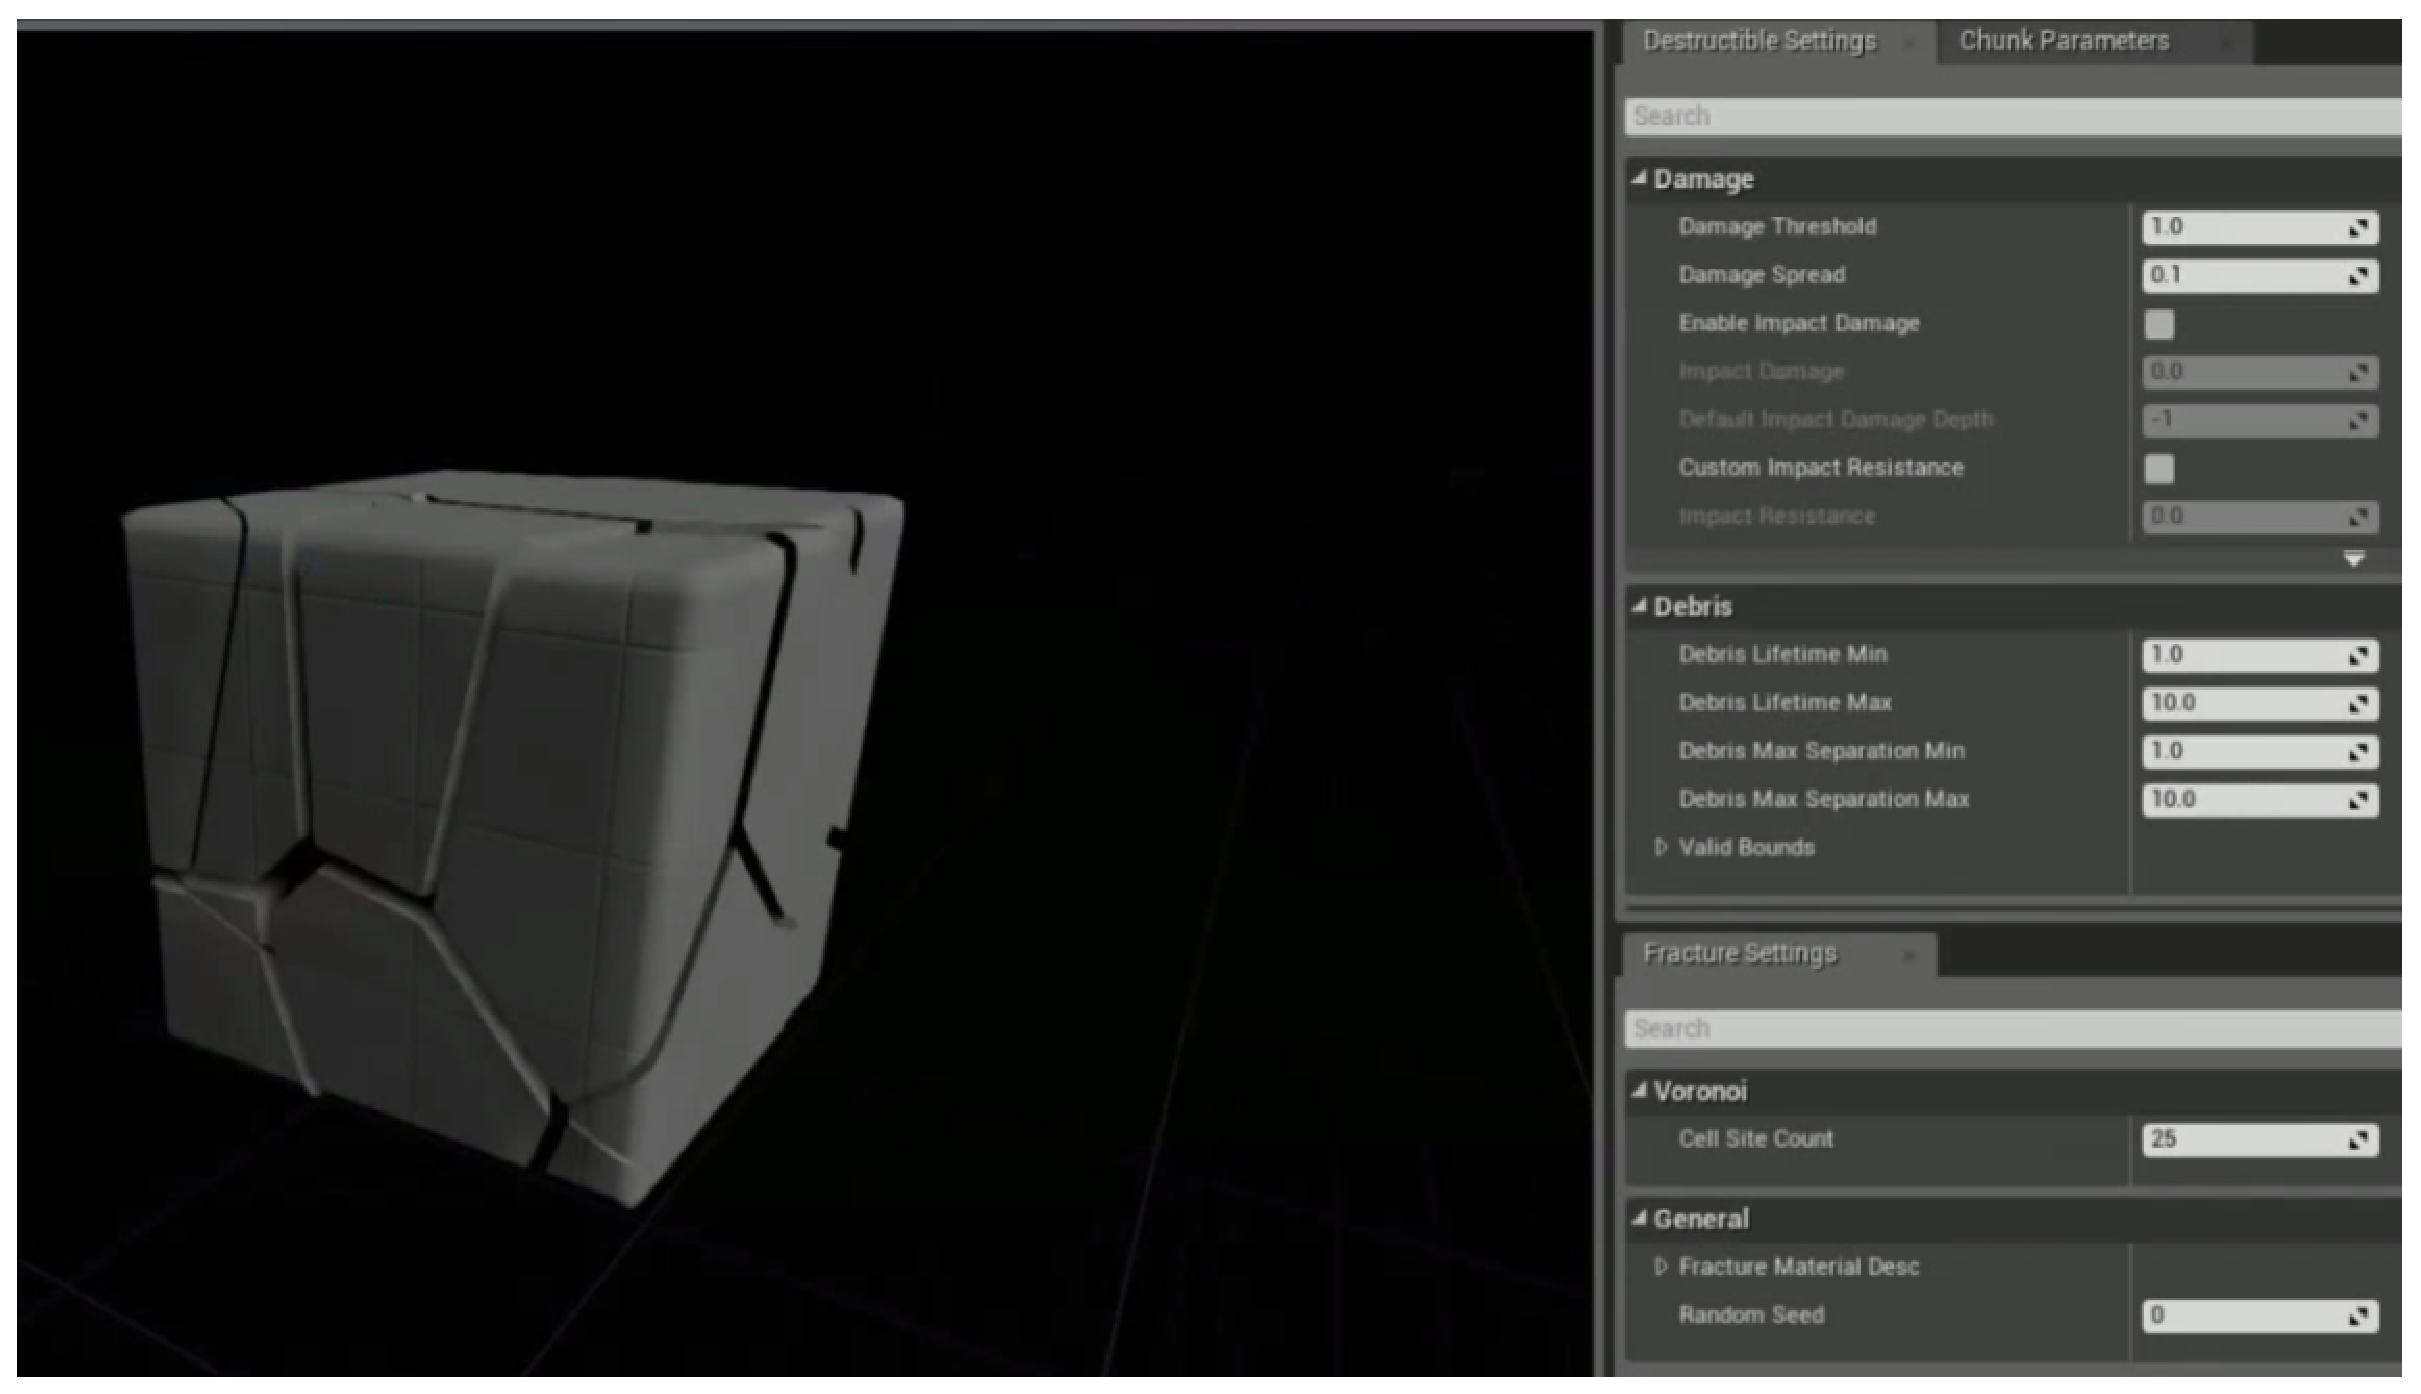
\includegraphics[width=1\textwidth]{destrEditor.eps}
	\caption{destructable mesh editor}
\end{figure}
\\
The system also offers many more features like damage thresholds,, a damage accumulator option or a damage spread factor.\\
Applying damage to an existing object is a simple and straightforward task. You can simply integrate an ``Apply Damage To'' or ''Apply Radial Damage to`` blueprint to your system and specify the needed parameters there.\\
\begin{figure}[ht]
	\centering
  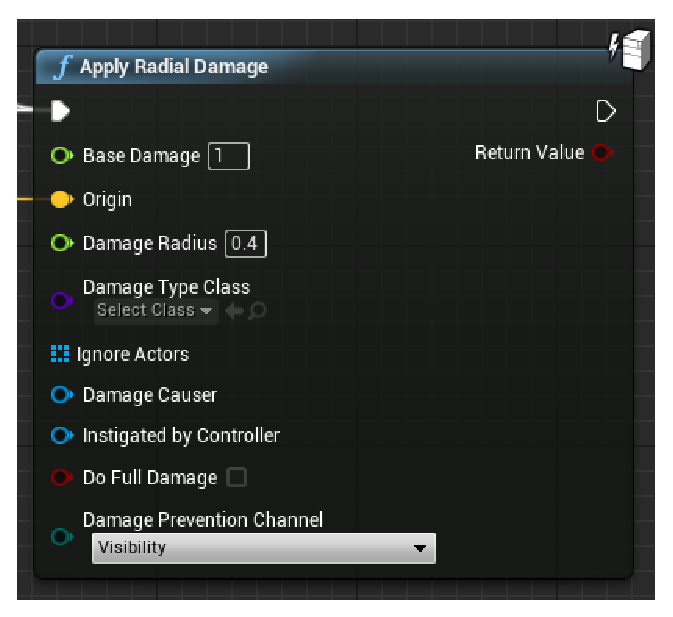
\includegraphics[width=0.7\textwidth]{radialDamage.eps}
	\caption{radial damage blueprint}
\end{figure}
\\
The next figure shows an example destruction using the described methods above.
\begin{figure}[ht]
	\centering
  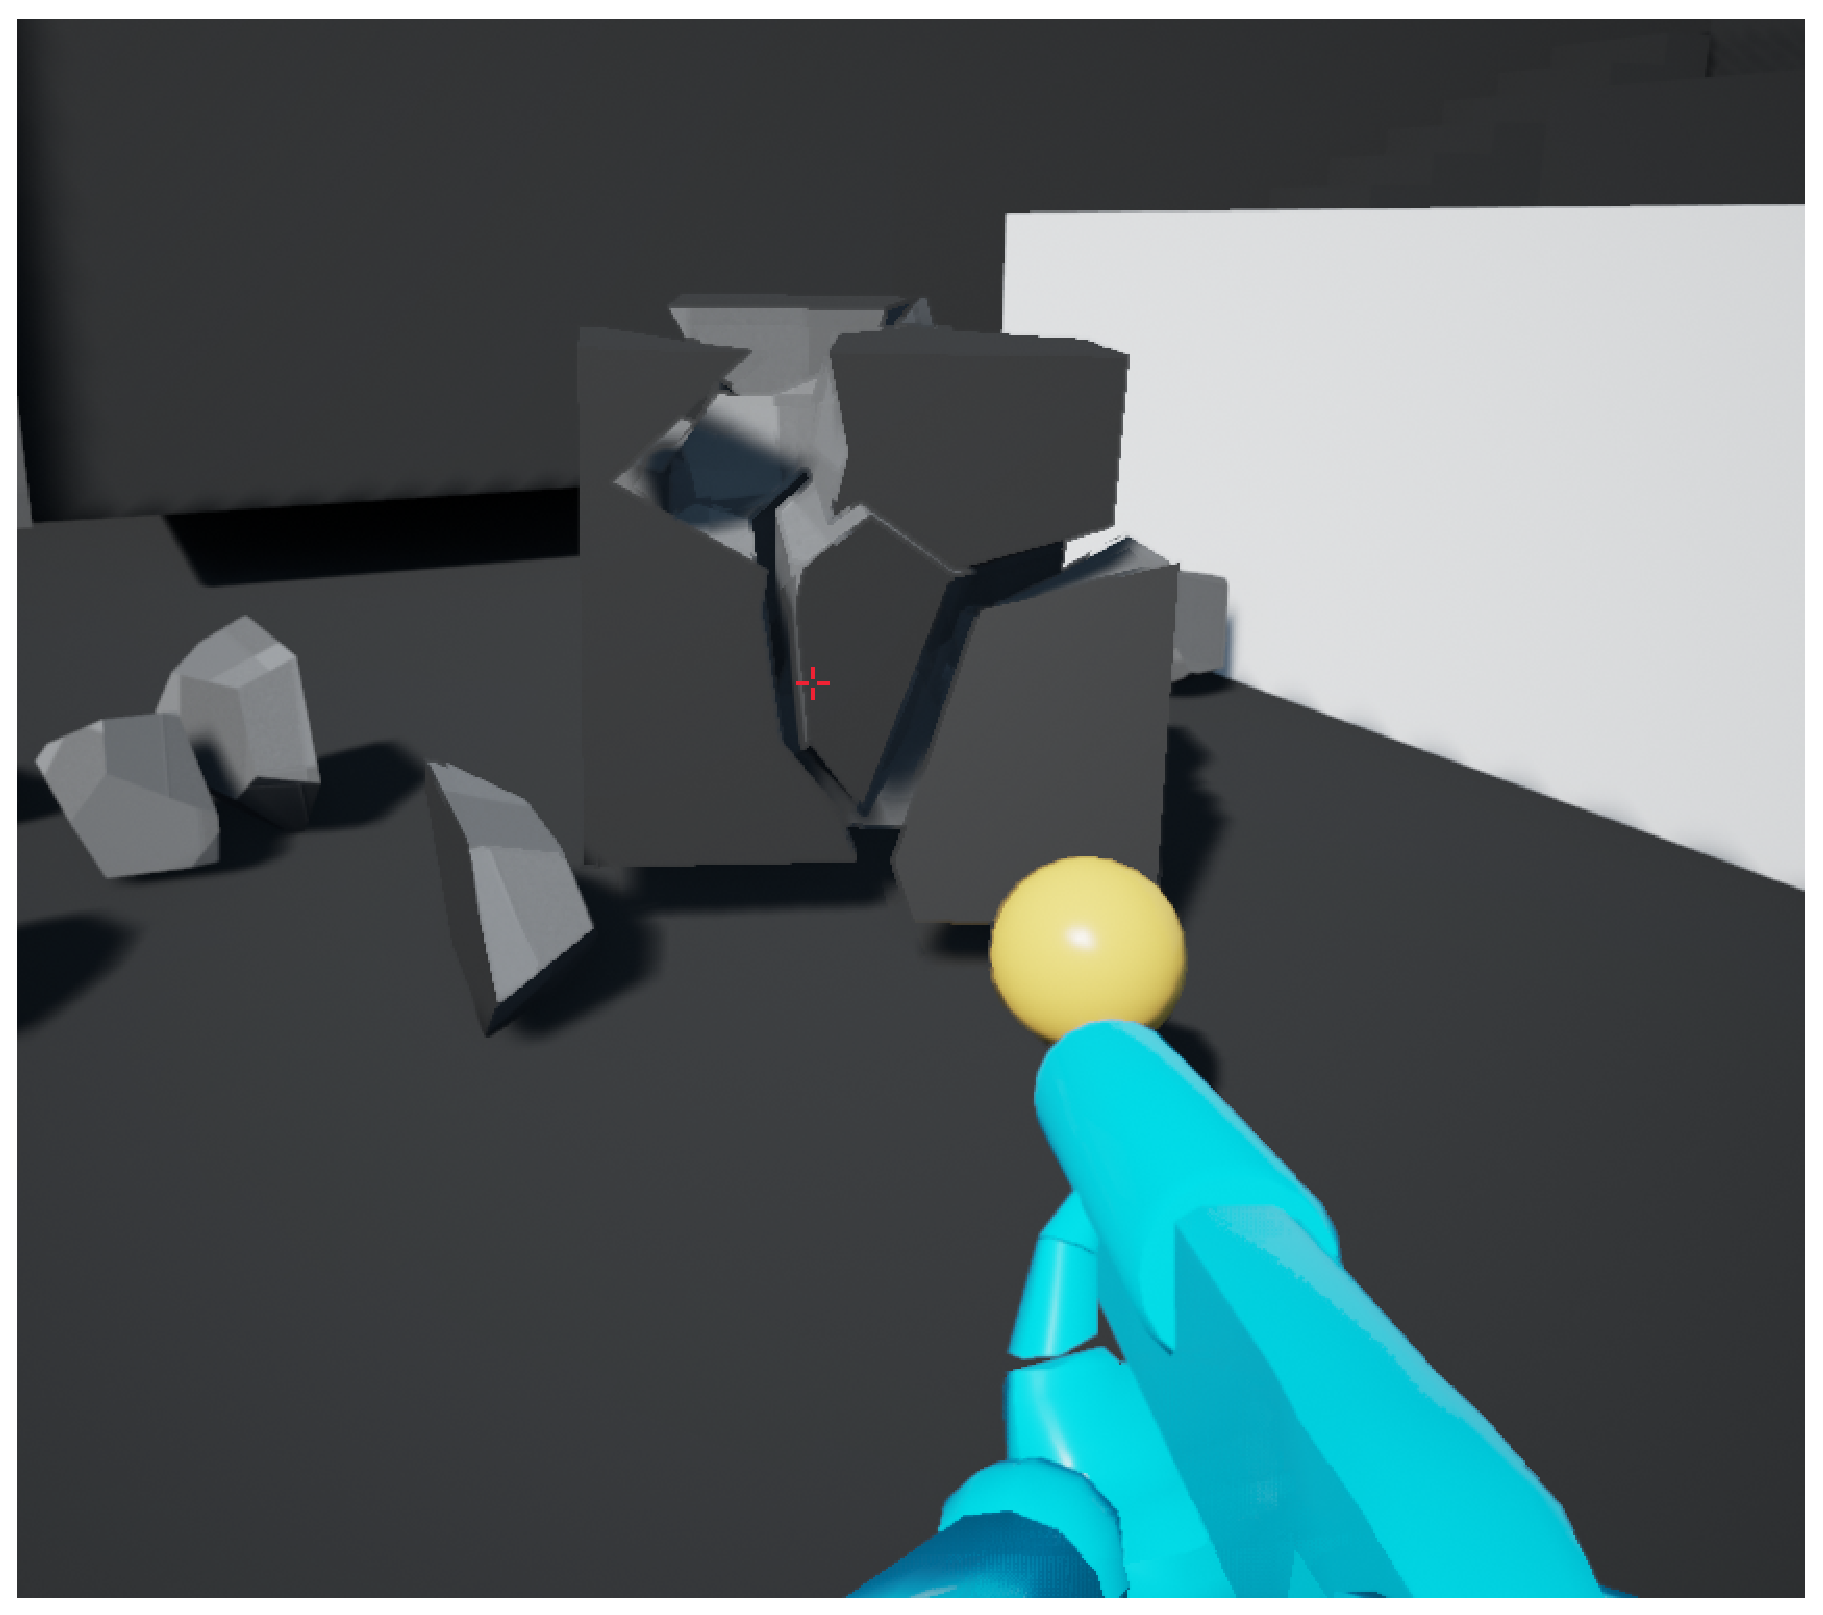
\includegraphics[width=0.7\textwidth]{destrExample.eps}
	\caption{destructable mesh example}
\end{figure}
\\
\end{document}
